\chapter{Ogólny zarys architektury systemu sterowania}
\label{cha:Ogolny_zarys_architektury_systemu_sterowania}

\begin{figure}[!htb]
	\centering
	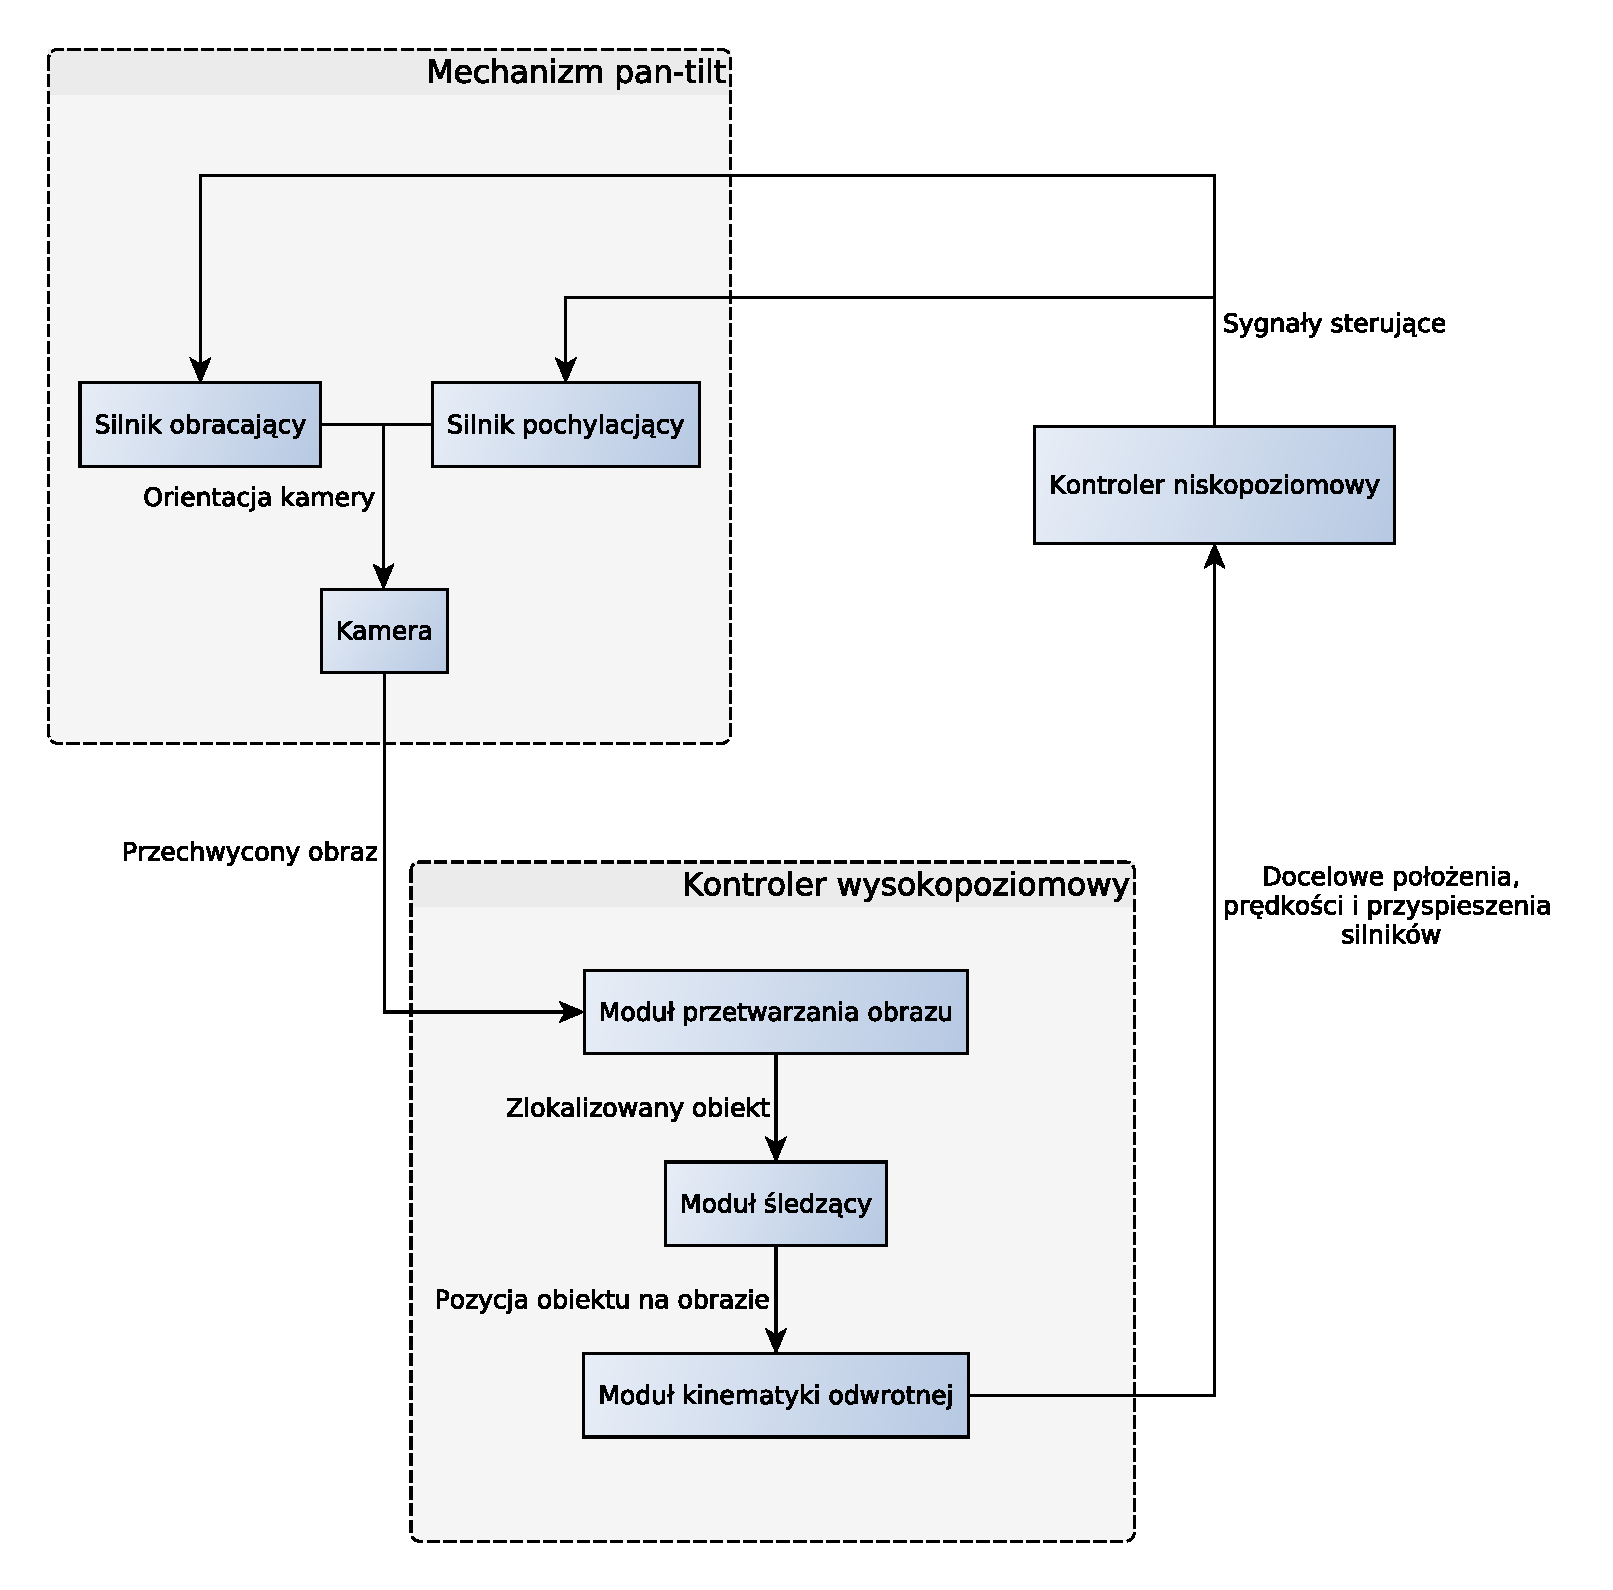
\includegraphics[width=9cm]{Images/system_overview.eps} 
	\captionsource{Schemat funkcjonalny systemu sterowania automatycznej głowicy śledzącej}{opracowanie własne}
\end{figure}

Na powyższym diagramie przedstawiona została ogólna zasada działania systemu sterowania. System składa się z następujących elementów:
\begin{enumerate}
	\item Mechanizm pan-tilt - realizacja funkcji orientowania kamery w celu uzyskania odpowiedniego pola widzenia
	\begin{enumerate}
		\item Silnik obracający
		\item Silnik pochylający
		\item Kamera wizyjna - główny sensor dostarczający danych wejściowych	
	\end{enumerate}	 
	\item Kontroler wysokopoziomowy - przetwarzanie dane wejściowych i określenie na ich podstawie parametrów pracy silników mechanizmu pan-tilt
	\begin{enumerate}
		\item Moduł przetwarzania obrazów - przeprowadzenie analizy obrazu z kamery wizyjnej, polegającej na wstępnej obróbce oraz lokalizacji obiektu zainteresowania
		\item Moduł śledzący - predykcji parametrów kinematycznych obiektu zainteresowania na podstawie pomiarów (w postaci współrzędnych obiektu na obrazie) oraz
			  estymacja jego przyszłego położenia
		\item Moduł kinematyki odwrotnej - obliczenie wartości współrzędnych złączowych mechanizmu pan-tilt na podstawie położenia obiektu zainteresowania
	\end{enumerate}
	\item Kontroler niskopoziomowy - konwersja docelowych parametrów kinematycznych do sygnałów sterujących
\end{enumerate}

